\chapter{Results and Discussion}

\section{Overview}

This chapter presents the results from the experiments described in Chapters 3 and 4. The main purpose is to examine whether the prompt families used in this project can reduce indicators of over-correction risk while still maintaining grammatical correction accuracy.

The chapter is organised around the six experiments carried out in the project. Experiment 1 selects the strongest prompt variant within each prompt family. Experiment 2 compares the selected baseline, instruction-constrained, role-based, and few-shot prompts. Experiment 3 examines whether sentence length affects correction behaviour. Experiment 4 checks the robustness of the OCI calculation. Experiment 5 considers the relationship between ERRANT $F_{0.5}$ and OCI. Experiment 6 then uses selected examples to examine possible over-correction behaviour in more detail.

Throughout this chapter, ERRANT $F_{0.5}$ is used as the main measure of grammatical correction quality. A higher $F_{0.5}$ score means that the model output is closer to the reference correction, with precision given more importance than recall. OCI, defined in Chapter 4, is used as the main indicator of over-correction risk. For this reason, the most suitable prompt is not simply the one with the highest $F_{0.5}$ score. It is the prompt that provides strong correction performance while limiting unnecessary rewriting.

It is important to interpret $F_{0.5}$ and OCI as measuring different aspects of correction behaviour. ERRANT focuses on agreement with a reference correction, while OCI indicates over-correction risk. OCI is therefore not treated as a perfect or direct measure of whether every edit is unnecessary. Some outputs with higher source-output change may still be reasonable if the original sentence contains several serious errors. Because of this, OCI is considered together with $F_{0.5}$, edit distance, qualitative examples, and sentence-level patterns rather than being used on its own.

\section{Experiment 1: Prompt Refinement}

\subsection{Purpose}

Experiment 1 was used to identify the strongest prompt variant within each prompt family before carrying out the main comparison. This step was needed because even small changes in prompt wording can affect how much an LLM edits learner writing. Two prompts may look similar but still lead to different levels of grammatical correction and different degrees of preservation of the original sentence.

\subsection{Implementation}

This experiment used 500 learner sentences from the prepared W\&I + LOCNESS subset. Each sentence was processed with the baseline prompt and with several variants from the instruction-constrained, role-based, and few-shot prompt families. For every output, ERRANT precision, recall, $F_{0.5}$, and OCI were calculated.

The aim of this stage was to select candidates for the main comparison, not to draw the final conclusions. The strongest prompt from each prompt family was therefore carried forward into Experiment 2, while the baseline prompt was kept as the control condition.

\subsection{Results}

\begin{table}[htbp]
    \centering
    \caption{Prompt refinement results for Experiment 1 -- all variants}
    \label{tab:exp1_prompt_refinement}
    \renewcommand{\arraystretch}{1.15}
    \begin{adjustbox}{max width=\textwidth}
    \begin{tabular}{lrrrr}
        \toprule
        \textbf{Condition} & \textbf{Precision} & \textbf{Recall} & \textbf{$F_{0.5}$} & \textbf{OCI (\%)} \\
        \midrule
        Baseline       & 42.71 & 52.32 & 44.34 & 1.40 \\
        \addlinespace
        Instruction v1 & 42.15 & 52.63 & 43.90 & 1.50 \\
        Instruction v2 & 53.54 & 39.01 & 49.83 & 0.98 \\
        Instruction v3 & 50.60 & 43.24 & 48.94 & 1.06 \\
        Instruction v4 & 52.82 & 39.63 & 49.52 & 1.05 \\
        \addlinespace
        Role v1        & 42.18 & 52.32 & 43.88 & 1.37 \\
        Role v2        & 44.77 & 50.77 & 45.85 & 1.36 \\
        Role v3        & 54.15 & 36.33 & 49.31 & 1.06 \\
        Role v4        & 55.03 & 38.39 & 50.64 & 1.05 \\
        \addlinespace
        Few-shot v1    & 44.37 & 51.29 & 45.60 & 1.51 \\
        Few-shot v2    & 45.27 & 51.39 & 46.38 & 1.49 \\
        Few-shot v3    & 45.49 & 52.01 & 46.66 & 1.54 \\
        Few-shot v4    & 54.47 & 43.34 & 51.81 & 1.12 \\
        \bottomrule
    \end{tabular}
    \end{adjustbox}
\end{table}

The baseline prompt achieved an $F_{0.5}$ score of 44.34 and an OCI of 1.40\%. Among the instruction-constrained prompts, Instruction v2 achieved the lowest OCI, 0.98\%, and an $F_{0.5}$ score of 49.83. Instruction v4 produced a very similar $F_{0.5}$ score, 49.52, with OCI of 1.05\%. Role v4 achieved $F_{0.5}$ of 50.64 and OCI of 1.05\%. Few-shot v4 achieved the highest $F_{0.5}$ score in this experiment, 51.81, with OCI of 1.12\%.

\subsection{Discussion}

The refinement results show that prompt wording has a measurable effect on correction behaviour. The baseline result is useful mainly as a reference point: a simple request to correct grammar does not reliably produce the most selective correction pattern.

Within the instruction-constrained family, Instruction v2 produced the lowest OCI among the instruction variants, while Instruction v4 produced a comparable accuracy profile. Instruction v4 was retained for the later comparison because it stated the minimal-edit constraint more explicitly, including tone, style, vocabulary, and unnecessary word addition or removal. Although Instruction v2 had a small numerical advantage in OCI, Instruction v4 better matched the final prompt design used for the main experiment.

The role-based prompts show a similar selection issue. Role v3 had marginally lower OCI, but Role v4 achieved stronger correction performance, making it the better role-based candidate for subsequent experiments. Few-shot v4 was the most accuracy-oriented variant. It achieved the highest $F_{0.5}$, suggesting that examples helped the model follow the expected correction format. Its OCI was slightly higher than the best instruction-constrained and role-based variants, suggesting a small increase in over-correction risk.

These results justify the final candidate set used in the main strategy comparison: Instruction v4, Role v4, Few-shot v4, and the baseline. The key limitation of Experiment 1 is that it is a refinement stage. It identifies strong candidates, but it does not by itself prove that one prompt family is generally superior. The later experiments are therefore needed to test whether the selected prompts remain strong under final comparison, sentence-length variation, and alternative OCI weighting schemes.

\section{Experiment 2: Comparison of Prompting Strategies}

\subsection{Purpose}

Experiment 2 compares the final prompting strategies selected in Experiment 1 in order to evaluate how different prompt designs influence the balance between grammatical correction performance and over-correction risk.

The aim is not only to identify which prompt achieves the highest correction score, but also to analyse how each strategy affects editing behaviour. In particular, the experiment examines whether improvements in ERRANT $F_{0.5}$ are associated with higher or lower over-correction risk, as estimated using OCI and supported by edit distance. This allows the analysis to distinguish between accuracy-oriented and more conservative correction strategies.

\subsection{Implementation}

The same 500 learner sentences were processed under four prompt conditions: baseline, instruction-constrained, role-based, and few-shot. The instruction-constrained, role-based, and few-shot prompts correspond to the refined variants selected in Experiment 1.

Outputs were evaluated using a two-branch framework. ERRANT precision, recall, and $F_{0.5}$ were used to measure agreement with reference corrections. OCI was used to estimate over-correction risk. Edit distance was also reported as a direct surface-change measure. This design enabled comparison between how many reference edits were attempted, how reliable those edits were, overall correction performance, and how much the sentence was altered.

Since each sentence was evaluated under all prompt conditions, paired comparisons were also used to assess whether OCI differences were consistent across inputs.

\subsection{Results}

\begin{table}[htbp]
    \centering
    \caption{Comparison of final prompt strategies for Experiment 2}
    \label{tab:exp2_strategy_comparison}
    \renewcommand{\arraystretch}{1.15}
    \begin{adjustbox}{max width=\textwidth}
    \begin{tabular}{lrrrrrr}
        \toprule
        \textbf{Condition} & \textbf{Precision} & \textbf{Recall} & \textbf{$F_{0.5}$} & \textbf{Mean OCI} & \textbf{OCI (\%)} & \textbf{Edit Dist.} \\
        \midrule
        Baseline    & 40.98 & 52.73 & 42.89 & 0.01678 & 1.68 & 6.70 \\
        Instruction & 52.82 & 39.63 & 49.52 & 0.01053 & 1.05 & 5.64 \\
        Role        & 55.03 & 38.39 & 50.64 & 0.01050 & 1.05 & 5.52 \\
        Few-shot    & 54.47 & 43.34 & 51.81 & 0.01119 & 1.12 & 5.67 \\
        \bottomrule
    \end{tabular}
    \end{adjustbox}
\end{table}

\begin{figure}[htbp]
    \centering
    
\includegraphics[width=\textwidth]{figures/figure_5_1_f05_vs_oci.png}
    \caption{Relationship between ERRANT $F_{0.5}$, mean OCI, precision, and recall across prompt conditions}
    \label{fig:f05_oci_tradeoff}
\end{figure}

\begin{figure}[htbp]
    \centering
    
\includegraphics[width=\textwidth]{figures/figure_5_2_prompt_strategy_comparison.png}
    \caption{Prompt strategy comparison using precision, recall, ERRANT $F_{0.5}$, and mean OCI}
    \label{fig:prompt_strategy_comparison}
\end{figure}

The baseline prompt performed worst overall, achieving the lowest $F_{0.5}$ score, 42.89, and the highest mean OCI, 0.01678. Although it obtained the highest recall, 52.73, its low precision, 40.98, indicates that many of its edits did not correspond to reference corrections.

All structured prompts improved $F_{0.5}$ while reducing OCI. Instruction-constrained prompting increased $F_{0.5}$ to 49.52 and reduced mean OCI to 0.01053. Role-based prompting achieved the highest precision, 55.03, an $F_{0.5}$ score of 50.64, and the lowest mean OCI, 0.01050, along with the lowest average edit distance, 5.52. Few-shot prompting achieved the highest $F_{0.5}$ score, 51.81, and the highest recall among the structured prompts, 43.34, but also produced a higher mean OCI, 0.01119, than instruction-constrained and role-based prompting.

To examine whether the OCI reductions were consistent across sentences, paired sentence-level comparisons were performed between the baseline and each structured prompt. Since each sentence was corrected under every prompt condition, a paired design was appropriate. Table~\ref{tab:exp2_paired_oci_tests} reports the mean OCI reduction, Wilcoxon signed-rank test result, and paired Cohen's $d_z$ effect size. Positive mean differences indicate lower OCI for the structured prompt than for the baseline.

\begin{table}[htbp]
    \centering
    \caption{Paired sentence-level OCI reductions relative to the baseline}
    \label{tab:exp2_paired_oci_tests}
    \renewcommand{\arraystretch}{1.15}
    \begin{adjustbox}{max width=\textwidth}
    \begin{tabular}{lrrrrrr}
        \toprule
        \textbf{Comparison} & \textbf{$n$} & \textbf{Baseline OCI} & \textbf{Prompt OCI} & \textbf{Mean reduction} & \textbf{$p$} & \textbf{$d_z$} \\
        \midrule
        Baseline vs Instruction & 500 & 0.01678 & 0.01053 & 0.00626 & $< .001$ & 0.25 \\
        Baseline vs Role        & 500 & 0.01678 & 0.01050 & 0.00629 & $< .001$ & 0.32 \\
        Baseline vs Few-shot    & 500 & 0.01678 & 0.01119 & 0.00559 & $< .001$ & 0.20 \\
        \bottomrule
    \end{tabular}
    \end{adjustbox}
\end{table}

All three reductions were statistically significant under a one-sided Wilcoxon signed-rank test ($p < .001$). The effect sizes are small to moderate, indicating that structured prompting shifts model behaviour consistently, but does not completely eliminate over-correction risk.

\subsection{Discussion}

Experiment 2 provides the main quantitative comparison for the dissertation. It shows how the selected prompts differ not only in ERRANT performance, but also in direct surface change, measured through edit distance, and over-correction risk, measured through OCI.

The baseline prompt behaves inefficiently under the ERRANT evaluation. Its recall is the highest at 52.73, so it attempts many edits, but its precision is only 40.98. This produces the lowest $F_{0.5}$ score, 42.89, and the highest mean OCI, 0.01678. In practical terms, the generic grammar-correction request encourages frequent modifications without enough control over whether those edits match the reference correction or preserve the learner's original expression.

The structured prompts behave differently from the baseline and from each other. Instruction-constrained prompting produces a clear reduction in OCI, from 0.01678 to 0.01053, while improving $F_{0.5}$ from 42.89 to 49.52. Its recall, 39.63, is lower than both the baseline and few-shot prompts, suggesting a more conservative correction style. This is consistent with explicit constraints on rewriting reducing the number of corrections attempted, while still improving the reliability of the output compared with the baseline.

Few-shot prompting achieves the highest $F_{0.5}$ score, 51.81, and the highest recall among the structured prompts, 43.34. This indicates that it identifies and attempts to correct a larger proportion of reference edits than the instruction-constrained and role-based prompts. However, it also produces a higher mean OCI, 0.01119, and a higher edit distance, 5.67, than role-based prompting. This suggests that few-shot prompting adopts a broader correction scope, making more changes to the input sentence and producing slightly higher over-correction risk.

Importantly, the higher OCI for few-shot prompting should be interpreted cautiously. OCI does not decide whether every edit is pedagogically or grammatically unjustified. Some additional edits may be appropriate, especially where the original sentence contains multiple or interacting errors. The safer interpretation is therefore that few-shot prompting has a broader correction scope: it increases reference-edit coverage, as reflected in recall and $F_{0.5}$, while also increasing over-correction risk.

Role-based prompting provides the strongest balance between correction performance and editing restraint. It achieves the highest precision, 55.03, meaning that a greater proportion of its edits correspond to reference corrections. Although its $F_{0.5}$ score, 50.64, is slightly lower than few-shot prompting, the difference is small at 1.17 points. At the same time, role-based prompting achieves the lowest mean OCI, 0.01050, and the lowest average edit distance, 5.52. Together, these metrics suggest that role-based prompting applies fewer but more targeted corrections.

The comparison between role-based and few-shot prompting is especially important. Few-shot prompting favours broader correction coverage, as shown by its higher recall and highest $F_{0.5}$. Role-based prompting favours selectivity, as shown by its higher precision, lower OCI, and lower edit distance. This means that the two prompts should not be interpreted simply as ``better'' or ``worse''. Instead, they represent different correction behaviours. Few-shot prompting is more accuracy-oriented under ERRANT evaluation, while role-based prompting is more suitable for minimal-edit or learner-facing correction settings where preserving the learner's original wording is important.

The paired OCI analysis adds a further qualification. The structured prompts do not only appear better at aggregate level; their lower OCI values are statistically reliable across the 500 paired sentences. However, the effect sizes are small to moderate. This means that prompt engineering produces a consistent behavioural shift, but it does not fully control over-correction risk. The practical value of the result comes from the combination of improved $F_{0.5}$ and reduced OCI, rather than from OCI reduction alone.

Experiment 2 therefore suggests that prompt engineering can make LLM-based GEC more selective. The role-based prompt gives the best balance in this comparison because it combines the highest precision, strong $F_{0.5}$, the lowest OCI, and the lowest edit distance. Few-shot prompting is still useful when correction coverage is the priority, but its higher OCI suggests greater over-correction risk.

\section{Experiment 3: Sentence-Length Effects}

\subsection{Purpose}

Experiment 3 investigated whether sentence length affects correction performance and over-correction risk. This is important because long learner sentences may contain several interacting grammatical issues, creating more opportunities for both necessary correction and broader rewriting.

\subsection{Implementation}

The experiment used a separate balanced subset of 450 sentences for the sentence-length analysis. Sentences were divided into three length categories: short sentences of 10 words or fewer, medium sentences of 11--20 words, and long sentences of more than 20 words. Each category contained 150 sentences. The four prompt strategies were evaluated separately within each length group. ERRANT $F_{0.5}$ was used to measure correction accuracy, while mean OCI was used to indicate over-correction risk.

\subsection{Results}

\begin{table}[htbp]
    \centering
    \caption{Sentence-length results for Experiment 3}
    \label{tab:exp3_length_results}
    \renewcommand{\arraystretch}{1.15}
    \begin{adjustbox}{max width=\textwidth}
    \begin{tabular}{llrr}
        \toprule
        \textbf{Condition} & \textbf{Length group} & \textbf{$F_{0.5}$} & \textbf{OCI (\%)} \\
        \midrule
        Baseline    & Short  & 42.11 & 2.76 \\
        Baseline    & Medium & 46.18 & 2.90 \\
        Baseline    & Long   & 37.11 & 5.61 \\
        \addlinespace
        Instruction & Short  & 48.55 & 1.77 \\
        Instruction & Medium & 52.50 & 2.23 \\
        Instruction & Long   & 43.13 & 4.23 \\
        \addlinespace
        Role        & Short  & 47.57 & 1.95 \\
        Role        & Medium & 57.19 & 2.20 \\
        Role        & Long   & 43.37 & 4.10 \\
        \addlinespace
        Few-shot    & Short  & 49.81 & 1.58 \\
        Few-shot    & Medium & 58.24 & 2.34 \\
        Few-shot    & Long   & 44.85 & 4.52 \\
        \bottomrule
    \end{tabular}
    \end{adjustbox}
\end{table}

\begin{figure}[htbp]
    \centering
    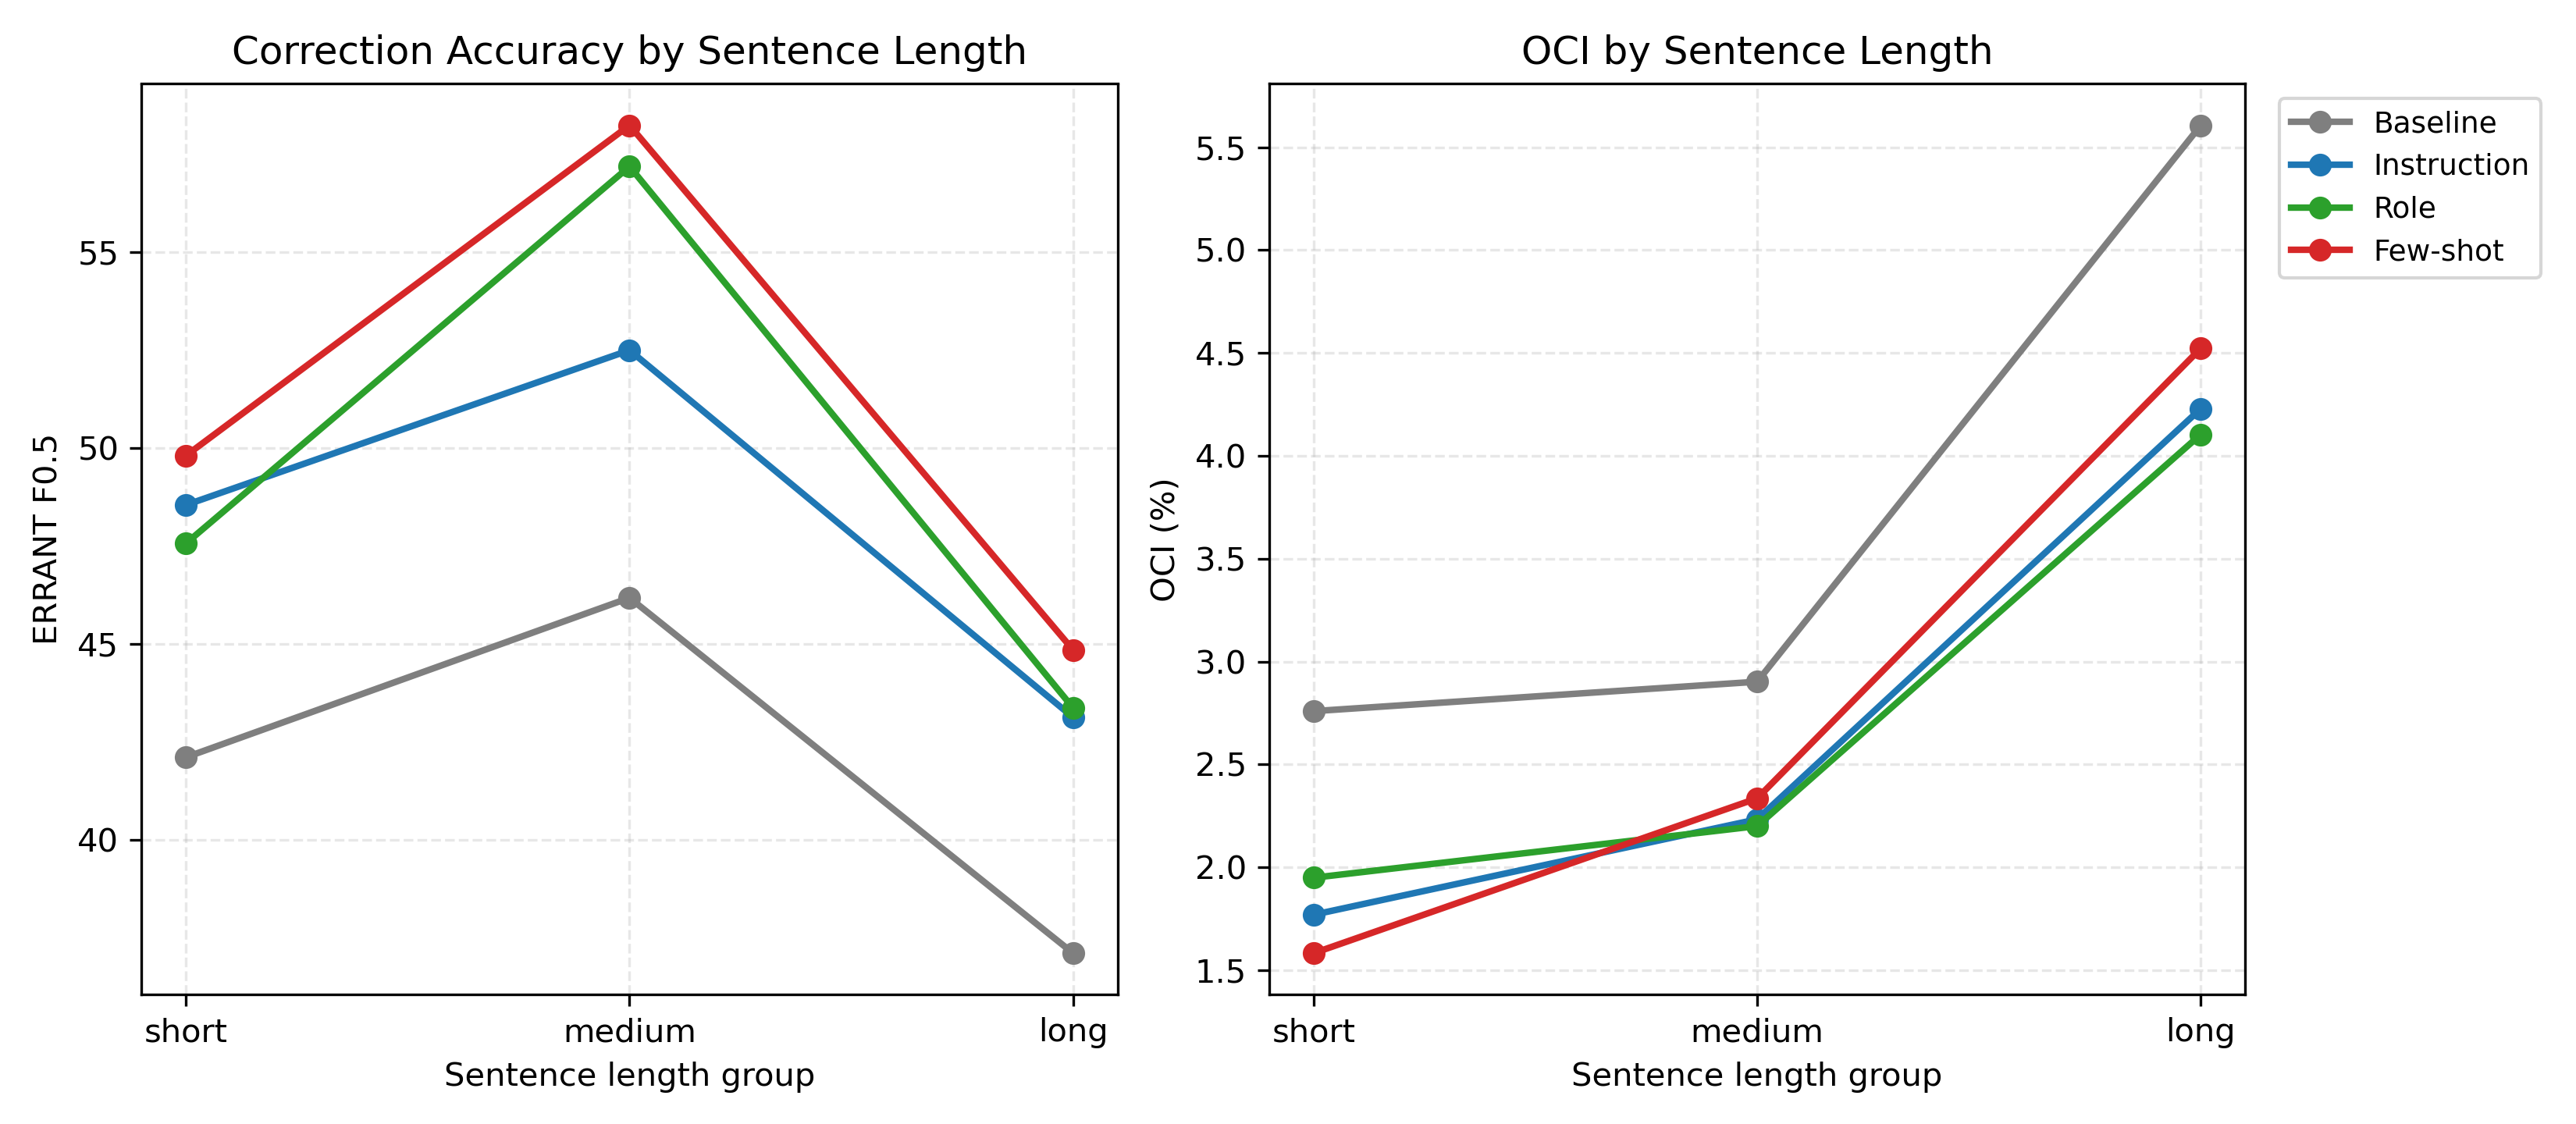
\includegraphics[width=\textwidth]{figures/figure_5_3_sentence_length_all_values.png}
    \caption{Sentence-length effects on correction accuracy and OCI}
    \label{fig:sentence_length_effects}
\end{figure}

Medium-length sentences produced the strongest $F_{0.5}$ scores across all prompt conditions. Few-shot prompting achieved the highest score in this group, 58.24, followed by role-based prompting at 57.19. Long sentences were the most difficult category. The baseline fell to 37.11 $F_{0.5}$ and reached 5.61\% OCI, while every non-baseline prompt still remained above 4\% OCI for long sentences.

\subsection{Discussion}

The sentence-length results suggest that over-correction risk is influenced by input complexity as well as prompt design. Medium-length sentences appear to provide enough context for grammatical correction while remaining short enough to avoid major structural rewriting. This helps explain why medium sentences produced the highest $F_{0.5}$ values.

Short sentences produced lower OCI values than long sentences, but they did not always produce the highest correction scores. Short inputs often contain fewer grammatical cues, so the model has less context for deciding whether an edit is required. This can lead either to under-correction or to additional changes with limited apparent utility.

Long sentences remain the main challenge. Their higher OCI values suggest greater over-correction risk when the input is longer. This is consistent with longer sentences creating more opportunities for reorganisation, paraphrasing, or accumulated local edits. The role-based prompt achieved the lowest OCI for long sentences, 4.10\%, suggesting that role-based framing remains the most restrained under complex input conditions. However, the increase in OCI across all prompts suggests that future systems may benefit from length-adaptive prompts that place stronger emphasis on preserving structure for longer inputs.

This result limits the generality of the main finding. Long and complex learner sentences remain difficult because the model must decide between local correction and sentence-level restructuring. The experiments suggest that current prompts can guide this decision, but cannot fully control it.

\section{Experiment 4: Robustness of the OCI Metric}

\subsection{Purpose}

Experiment 4 tested whether OCI-based conclusions were stable under alternative weighting schemes. This was necessary because OCI is a composite indicator, and its usefulness depends on whether prompt rankings remain broadly consistent when component weights are changed.

\subsection{Implementation}

The experiment reused the Experiment 2 style metrics and recalculated the formula under five weighting schemes: default, edit-heavy, style-heavy, similarity-heavy, and equal weights. The same utility adjustment was then applied in each case. For each weighting scheme, prompt conditions were ranked by mean OCI, where rank 1 indicates the lowest over-correction risk.

\subsection{Results}

\begin{table}[htbp]
    \centering
    \caption{OCI prompt rankings under alternative weighting schemes}
    \label{tab:exp4_oci_robustness}
    \renewcommand{\arraystretch}{1.15}
    \begin{adjustbox}{max width=\textwidth}
    \begin{tabular}{lllll}
        \toprule
        \textbf{Weighting scheme} & \textbf{Rank 1} & \textbf{Rank 2} & \textbf{Rank 3} & \textbf{Rank 4} \\
        \midrule
        Default           & Role (0.0105)        & Instruction (0.0105) & Few-shot (0.0112) & Baseline (0.0168) \\
        Edit-heavy        & Role (0.0111)        & Instruction (0.0112) & Few-shot (0.0114) & Baseline (0.0160) \\
        Style-heavy       & Role (0.0097)        & Instruction (0.0098) & Few-shot (0.0107) & Baseline (0.0167) \\
        Similarity-heavy  & Instruction (0.0081) & Role (0.0082)        & Few-shot (0.0085) & Baseline (0.0134) \\
        Equal weights     & Role (0.0087)        & Instruction (0.0087) & Few-shot (0.0093) & Baseline (0.0149) \\
        \bottomrule
    \end{tabular}
    \end{adjustbox}
\end{table}

\begin{figure}[htbp]
    \centering
    
\includegraphics[width=0.86\textwidth]{figures/figure_5_4_oci_robustness.png}
    \caption{OCI ranking stability across weighting schemes}
    \label{fig:oci_robustness}
\end{figure}

The OCI rankings were highly stable. The baseline was ranked last under every weighting scheme, indicating that it produced the highest over-correction risk. Few-shot prompting was consistently ranked third. Instruction-constrained and role-based prompting occupied the top two positions under every scheme. Role-based prompting ranked first in four of the five schemes, while instruction-constrained prompting ranked first under the similarity-heavy scheme.

\subsection{Discussion}

The robustness analysis strengthens the OCI-based comparison. If the prompt rankings had changed substantially under different weights, the metric would be difficult to interpret. Instead, the broad pattern remains stable: baseline is the least controlled condition, few-shot is more interventionist than instruction-constrained and role-based prompting, and role-based and instruction-constrained prompting form the most conservative pair.

The small difference between instruction-constrained and role-based prompting should therefore be interpreted cautiously. Their OCI scores are close, and their rank changes only under the similarity-heavy setting. This is consistent with Experiment 2, where role-based prompting had slightly lower edit distance but instruction-constrained prompting had a very similar OCI value.

At the same time, this experiment does not make OCI objective in an absolute sense. The weighting schemes test robustness, but the metric still reflects design choices. It is strongest when used for relative comparison between prompts under the same experimental conditions. It is less appropriate as a standalone judgement that a particular individual sentence has definitely been over-corrected.

\section{Experiment 5: Accuracy and Over-Correction Trade-Off}

\subsection{Purpose}

Experiment 5 examined the relationship between correction performance and over-correction risk. The aim was to determine whether higher grammatical accuracy necessarily comes with higher OCI, or whether some prompts can achieve a better balance.

\subsection{Implementation}

The experiment merged the ERRANT scores and mean OCI values from Experiment 2. Each prompt condition was represented as one point in the trade-off space, with mean OCI on the x-axis and ERRANT $F_{0.5}$ on the y-axis. This made it possible to identify prompts that were weak, conservative, accuracy-oriented, or balanced.

\subsection{Results}

\begin{table}[htbp]
    \centering
    \caption{Trade-off between correction performance and over-correction risk}
    \label{tab:exp5_tradeoff}
    \renewcommand{\arraystretch}{1.15}
    \begin{adjustbox}{max width=\textwidth}
    \begin{tabular}{lrrrrl}
        \toprule
        \textbf{Condition} & \textbf{Precision} & \textbf{Recall} & \textbf{$F_{0.5}$} & \textbf{Mean OCI} & \textbf{Interpretation} \\
        \midrule
        Baseline    & 40.98 & 52.73 & 42.89 & 0.01678 & Weak/inefficient \\
        Instruction & 52.82 & 39.63 & 49.52 & 0.01053 & Conservative \\
        Role        & 55.03 & 38.39 & 50.64 & 0.01050 & Balanced \\
        Few-shot    & 54.47 & 43.34 & 51.81 & 0.01119 & Accuracy-oriented \\
        \bottomrule
    \end{tabular}
    \end{adjustbox}
\end{table}

The baseline prompt falls into the weakest region of the trade-off space. It has the lowest $F_{0.5}$ and the highest mean OCI, meaning that it is neither accurate nor controlled under these evaluation criteria. Few-shot prompting achieved the highest $F_{0.5}$ score, 51.81, but also had higher OCI than instruction-constrained and role-based prompting. Instruction-constrained prompting was the most conservative structured strategy, while role-based prompting produced the best overall balance.

\subsection{Discussion}

Experiment 5 brings the accuracy and OCI results together. The baseline prompt shows why high recall alone is not enough: it makes many edits, but still has weak $F_{0.5}$ and high OCI. The role-based prompt sits in the more useful part of the trade-off space because it keeps OCI low while maintaining strong correction performance.

Few-shot prompting is useful when reference-matching accuracy is prioritised. However, its higher OCI suggests that it is not the best option when preservation of learner wording is equally important. Instruction-constrained prompting is preferable when conservative editing is the main goal. Role-based prompting is the strongest compromise in this trade-off table because it sits between the conservative instruction-constrained prompt and the accuracy-oriented few-shot prompt.

The trade-off is therefore not a simple linear relationship where more accuracy always requires more rewriting. The baseline has both low $F_{0.5}$ and high OCI, indicating that extensive editing can be unproductive. The remaining trade-off is mainly between role-based and few-shot prompting: few-shot gains the highest $F_{0.5}$, while role-based prompting better preserves the source.

\section{Experiment 6: Qualitative Analysis}

\subsection{Purpose}

Experiment 6 provides sentence-level examples to explain the quantitative results. While $F_{0.5}$ and OCI show differences between prompt conditions, qualitative analysis helps show how potential over-correction appears in practice.

\subsection{Implementation}

The analysis compared baseline outputs with outputs from the role-based prompt, which was the strongest balanced condition in the quantitative experiments. Examples were selected from the generated outputs to illustrate common behaviours observed during evaluation: task-format failure, unnecessary paraphrasing, and style-changing rewriting.

\subsection{Results}

\begin{table}[htbp]
    \centering
    \caption{Qualitative examples of over-correction behaviour}
    \label{tab:qualitative_examples}
    \renewcommand{\arraystretch}{1.25}
    \begin{adjustbox}{max width=\textwidth}
    \begin{tabularx}{\textwidth}{
        >{\raggedright\arraybackslash}p{0.27\textwidth}
        >{\raggedright\arraybackslash}p{0.36\textwidth}
        >{\raggedright\arraybackslash}p{0.31\textwidth}
    }
        \toprule
        \textbf{Source} & \textbf{Baseline output} & \textbf{Role output} \\
        \midrule
        Personal experiences
        & I'm sorry, but I need the full sentence to provide a correction. Could you please provide the complete sentence?
        & Personal experience \\
        \addlinespace

        Public transport is not convenient for most of the people because every person wants to reach on time at his place but using public transport it is very difficult to reach on time.
        & Public transport is not convenient for most people because everyone wants to reach their destination on time, but using public transport makes it very difficult to do so.
        & Public transport is not convenient for most of the people because every person wants to reach on time at his place, but using public transport it is very difficult to reach on time. \\
        \addlinespace

        After walking for a lot of days, the survivors were worried, and thinking of how much they would still need to walk to find a city.
        & After walking for many days, the survivors were worried and thinking about how much farther they would need to walk to find a city.
        & After walking for a lot of days, the survivors were worried and thinking of how much they would still need to walk to find a city. \\
        \bottomrule
    \end{tabularx}
    \end{adjustbox}
\end{table}

\subsection{Discussion}

The first example shows task-format failure. Although ``Personal experiences'' is closer to a fragment or title than a full sentence, it is retained because the pipeline must still handle such inputs when they occur in the dataset. The baseline produces a conversational response instead of a corrected text span. This is problematic because the output is no longer a GEC correction. It also creates a large change from the source without providing useful grammatical feedback.

The second example shows unnecessary paraphrasing. The baseline output is fluent, but it changes ``every person'' to ``everyone'' and ``his place'' to ``their destination''. These changes improve idiomatic fluency, but they go beyond minimal grammatical correction. The role-based prompt preserves more of the learner's wording and structure.

The third example shows meaning-preserving but style-changing rewriting. The baseline changes ``thinking of how much they would still need to walk'' to ``thinking about how much farther they would need to walk''. This is not grammatically wrong, but it is more interventionist than necessary. The role-based output stays closer to the original sentence.

The qualitative analysis helps explain why the baseline can have high OCI without achieving high $F_{0.5}$. Potential over-correction is not only associated with correct grammatical edits. It can also be associated with refusals, invented context, paraphrasing, and fluency-driven rewriting.

These examples also show why automatic metrics need to be interpreted carefully. A fluent rewritten sentence may look better in isolation, but it can be less appropriate for learner-facing correction if it removes the learner's wording unnecessarily. Conversely, a minimal correction may preserve awkward phrasing that a human teacher might choose to discuss separately. This supports the use of prompt controls that specify the intended correction style rather than relying on a generic request for fluent English.

\section{Overall Discussion}

The results suggest that prompt engineering can reduce indicators of over-correction risk in this LLM-based GEC setup. The clearest evidence comes from Experiment 2, where all structured prompts improve $F_{0.5}$ and reduce OCI relative to the baseline.

The role-based prompt provides the best overall balance in these experiments. It achieves the highest precision, strong $F_{0.5}$, low OCI, and the lowest average edit distance. Instruction-constrained prompting is the most conservative alternative, while few-shot prompting is the most accuracy-oriented strategy.

Sentence length adds an important qualification. Long sentences remain difficult even under the stronger prompt conditions, suggesting that future systems may need length-aware or complexity-aware prompting.

The robustness analysis supports the OCI-based interpretation because the broad prompt ranking remains stable under alternative weighting schemes. This suggests that the main pattern is not caused by one specific weighting choice. However, OCI should still be interpreted as a comparative indicator of over-correction risk, not as a definitive judgement that every high-scoring sentence has been unnecessarily corrected.

The qualitative examples illustrate why ERRANT alone does not capture all relevant correction behaviour. A sentence may be fluent and grammatically acceptable while still raising over-correction concerns if it changes the learner's wording more than necessary. For learner-facing GEC, preserving the learner's intended expression is therefore an important evaluation concern alongside grammatical accuracy.

Across the six experiments, the research question can be answered with a qualified yes. Prompt engineering can reduce over-correction risk in this LLM-based GEC setting, especially through role-based and instruction-constrained prompts. However, the reduction is not uniform across all inputs, and long sentences remain challenging. The project therefore does not show that prompting eliminates over-correction. It shows that prompt design can shift the model towards a better balance between accuracy and restraint without changing the underlying model.

\section{Chapter Summary}

This chapter reported six experiments evaluating prompt-based reduction of over-correction risk in LLM-based GEC. Prompt refinement selected the strongest candidate from each prompt family. Strategy comparison showed that instruction-constrained, role-based, and few-shot prompting all improved $F_{0.5}$ while reducing OCI. Sentence-length analysis showed that long sentences remain the most difficult. OCI robustness analysis showed stable rankings across weighting schemes. Trade-off analysis identified role-based prompting as the best balance between accuracy and restraint. Qualitative analysis illustrated how potential over-correction appears in practical outputs.

The results indicate that prompt engineering can reduce over-correction risk while maintaining grammatical correction performance. Among the tested strategies, role-based prompting provides the strongest balance between grammatical accuracy and preservation of learner wording.
